\section{Vistas}
A continuación, se presentan algunos ejemplos de vistas creadas en el proyecto, junto con sus resultados y conclusiones.
\subsection{Vista de los alojamientos con mayor disponibilidad anual}
En esta consulta podemos ver los alojamientos con mayor disponibilidad anual.
La vista 'year\_availability' muestra los alojamientos con mayor disponibilidad durante todo el año en Málaga. Permite facilitar a los usuarios la identificación de opciones con una alta disponibilidad para reservar en cualquier época.\\A continuación se muestra el código de la vista y un fragmento de los resultados:

\begin{verbatim}
CREATE OR REPLACE VIEW year_availability AS
    SELECT name, availability_365
    FROM listings
    ORDER BY availability_365 DESC
\end{verbatim}

\begin{table}[h]
\centering
\resizebox{\textwidth}{!}{
\begin{tabular}{|l|l|r|}
\hline
\textbf{Nombre del alojamiento} & \textbf{Enlace del alojamiento} & \textbf{Disponibilidad anual} \\ \hline
EXCELENTE PISO CASCO HISTORICO & \href{https://www.airbnb.com/rooms/678778297636694785}{https://www.airbnb.com/rooms/678778297636694785} & 365 \\ \hline
Habitación acogedora cerca del centro de Málaga & \href{https://www.airbnb.com/rooms/634843206096078765}{https://www.airbnb.com/rooms/634843206096078765} & 365 \\ \hline
Modern and Sunny Loft Terrace closed to beach & \href{https://www.airbnb.com/rooms/26564973}{https://www.airbnb.com/rooms/26564973} & 365 \\ \hline
Charming apartment in Málaga near seabeach & \href{https://www.airbnb.com/rooms/819266217210297893}{https://www.airbnb.com/rooms/819266217210297893} & 365 \\ \hline
Welcoming apartment at the center of Málaga & \href{https://www.airbnb.com/rooms/617319758965018121}{https://www.airbnb.com/rooms/617319758965018121} & 365 \\ \hline
1 Bedrooms Apartment La Mundial & \href{https://www.airbnb.com/rooms/44010462}{https://www.airbnb.com/rooms/44010462} & 365 \\ \hline
Luxurious Apartment Gold Mile & \href{https://www.airbnb.com/rooms/790376052631156910}{https://www.airbnb.com/rooms/790376052631156910} & 365 \\ \hline
... & ... & ... \\ \hline
\end{tabular}
}
\caption{Alojamientos con mayor disponibilidad anual en Málaga.}
\end{table}

La vista 'year\_availability' proporciona una lista de alojamientos que permanecen disponibles durante todo el año, lo que puede ser útil para viajeros que buscan opciones flexibles en cuanto a fechas de estancia. Existe una gran cantidad de alojamientos con plena disponibilidad durante todo un año. Si consultamos la vista desde la última fila observaremos los alojamientos con disponibilidad más corta, que puede ser de gran utilidad para viajeros con planes más concretos o aquellos que buscan estancias más cortas.

\subsection{Vista de la disponibilidad y el precio diario de los listados}

Se creó una vista llamada 'listing\_availability\_price' para mostrar la disponibilidad y el precio diario de los listados. Con esta vista, los usuarios pueden obtener información sobre las fechas disponibles para cada alojamiento y su precio diario correspondiente. \\
A continuación se muestra el código de la vista y un fragmento de los resultados:

\begin{verbatim}
CREATE OR REPLACE VIEW listing_availability_price AS
SELECT l.listing_url, l.name, MIN(c.date) AS start_date, 
    MAX(c.date) AS end_date,
    ROUND(AVG(CAST(REGEXP_REPLACE(REPLACE(l.price, '$', ''),
        '[^\d.]', '', 'g') AS NUMERIC)), 2) AS price
FROM calendar c
JOIN listings l ON c.listing_id = l.id
WHERE c.available = 't'
GROUP BY l.id, l.name, l.price;
\end{verbatim}

\begin{table}[h]
\centering
\resizebox{\textwidth}{!}{
\begin{tabular}{|l|l|r|r|l|}
\hline
\textbf{URL} & \textbf{Nombre del alojamiento} & \textbf{Fecha de inicio} & \textbf{Fecha de fin} & \textbf{Precio diario} \\ \hline
\href{https://www.airbnb.com/rooms/31039156}{https://www.airbnb.com/rooms/31039156} & CENTRO HISTÓRICO 2 HABITACIONES LAZCANO & 2023-04-09 & 2023-09-30 & 103.00 \texteuro \\ \hline
\href{https://www.airbnb.com/rooms/854447844432131414}{https://www.airbnb.com/rooms/854447844432131414} & Bluemarine room for tour & 2023-04-03 & 2023-04-30 & 65.00 \texteuro \\ \hline
\href{https://www.airbnb.com/rooms/574649101626526498}{https://www.airbnb.com/rooms/574649101626526498} & Perfect Suite Train station & 2023-04-09 & 2023-06-29 & 76.00 \texteuro \\ \hline
\href{https://www.airbnb.com/rooms/749258261295533795}{https://www.airbnb.com/rooms/749258261295533795} & Nuevo loft - Piscina, Playa \& relax & 2023-04-09 & 2024-03-29 & 45.00 \texteuro \\ \hline
\href{https://www.airbnb.com/rooms/594786518117713438}{https://www.airbnb.com/rooms/594786518117713438} & La Perla de Málaga & 2023-04-02 & 2024-03-30 & 118.00 \texteuro \\ \hline
... & ... & ... & ... & ... \\ \hline
\end{tabular}
}
\caption{Disponibilidad y precio diario de los alojamientos en Málaga}
\end{table}

\newpage
\subsection{Vista del precio medio según el número de habitaciones}

Se creó una vista llamada 'price\_by\_bedrooms' para mostrar el precio medio según el número de habitaciones. Esto puede ser útil para los viajeros que deseen encontrar alojamientos que se ajusten a sus necesidades y presupuesto en función del tamaño del grupo con el que viajan. \\
A continuación se muestra el código de la vista y un fragmento de los resultados:

\begin{verbatim}
CREATE OR REPLACE VIEW price_by_bedrooms AS 
	SELECT bedrooms, 
    ROUND(AVG(CAST(REGEXP_REPLACE(price, '[^\d.]', '', 'g') 
        AS NUMERIC))) AS avg_price 
	FROM listings 
	GROUP BY bedrooms 
	ORDER BY avg_price DESC;
\end{verbatim}

\begin{table}[h]
\centering
\begin{tabular}{|r|r|}
\hline
\textbf{Número de Habitaciones} & \textbf{Precio Medio} \\ \hline
25 & 1285 \texteuro\\ \hline
24 & 1285 \texteuro\\ \hline
12 & 1106 \texteuro\\ \hline
11 & 676 \texteuro\\ \hline
10 & 600 \texteuro\\ \hline
15 & 564 \texteuro\\ \hline
8 & 561 \texteuro\\ \hline
9 & 465 \texteuro\\ \hline
7 & 442 \texteuro\\ \hline
5 & 428 \texteuro\\ \hline
6 & 413 \texteuro\\ \hline
3 & 292 \texteuro\\ \hline
4 & 277 \texteuro\\ \hline
2 & 213 \texteuro\\ \hline
1 & 146 \texteuro\\ \hline
\end{tabular}
\caption{Precio medio según el número de habitaciones de los alojamientos en Málaga.}
\end{table}
Se puede observar que los alojamientos con un número inusualmente alto de habitaciones, como 24 o 25 habitaciones, tienen precios medios excepcionalmente altos. Esto sugiere que los alojamientos de gran capacidad tienden a ser más costosos en promedio, lo cual es comprensible debido a su capacidad para acomodar a un gran número de personas.
\subsection{Vista de las tendencias de precios medios a lo largo de los años}

La vista 'price\_trends' se ha creado con el propósito de mostrar las tendencias de los precios medios de alojamientos a lo largo de los años. Esta información puede ser útil para los viajeros y propietarios de alojamientos, ya que proporciona una visión general de cómo han evolucionado los precios a lo largo del tiempo.
\\
A continuación se muestra el código de la vista y un fragmento de los resultados:

\begin{verbatim}
CREATE OR REPLACE VIEW price_trends AS 
SELECT TO_CHAR(date, 'YYYY-MM') AS year_month, 
ROUND(AVG(CAST(REGEXP_REPLACE(price, '[^\d.]', '', 'g') 
    AS NUMERIC))) AS avg_price 
    FROM calendar 
    GROUP BY TO_CHAR(date, 'YYYY-MM') 
    ORDER BY year_month;
\end{verbatim}

\begin{table}[h]
\centering
\begin{tabular}{|l|r|}
\hline
\textbf{Año-Mes} & \textbf{Precio Medio } \\ \hline
2023-03 & 196 \texteuro\\ \hline
2023-04 & 181 \texteuro\\ \hline
2023-05 & 174 \texteuro\\ \hline
2023-06 & 165 \texteuro\\ \hline
2023-07 & 184 \texteuro\\ \hline
2023-08 & 205 \texteuro\\ \hline
2023-09 & 195 \texteuro\\ \hline
2023-10 & 208 \texteuro\\ \hline
2023-11 & 197 \texteuro\\ \hline
2023-12 & 215 \texteuro\\ \hline
2024-01 & 215 \texteuro\\ \hline
2024-02 & 236 \texteuro\\ \hline
2024-03 & 265 \texteuro\\ \hline
\end{tabular}
\caption{Tendencias de precios medios a lo largo de los años en alojamientos de Málaga.}
\end{table}
\newpage
Los viajeros pueden utilizar esta información para planificar sus viajes en momentos que se ajusten a su presupuesto, mientras que los propietarios de alojamientos pueden tomar decisiones informadas sobre cómo ajustar sus tarifas según la demanda en diferentes períodos del año.

\subsection{Vista de las tendencias de disponibilidad en los próximos meses}
Se creó una vista llamada 'availability\_trends' para mostrar las tendencias de disponibilidad que se presentarán a lo largo de los próximos meses. Esta información es valiosa tanto para los viajeros como para los propietarios de alojamientos, ya que proporciona una visión general de la disponibilidad de alojamientos en diferentes períodos del tiempo.\\
A continuación se muestra el código de la vista y un fragmento de los resultados:
\begin{verbatim}
CREATE OR REPLACE VIEW availability_trends
 AS
 SELECT TO_CHAR(date, 'YYYY-MM') AS year_month,
    sum(
        CASE
            WHEN calendar.available = 't'::bpchar THEN 1
            ELSE 0
        END) AS available_listings,
    sum(
        CASE
            WHEN calendar.available = 'f'::bpchar THEN 1
            ELSE 0
        END) AS unavailable_listings
   FROM calendar
  GROUP BY TO_CHAR(date, 'YYYY-MM')
  ORDER BY year_month;
\end{verbatim}
\begin{table}[h]
\centering

\begin{tabular}{|l|r|r|}
\hline
\textbf{Año-Mes} & \textbf{Alojamientos Disponibles} & \textbf{Alojamientos No Disponibles} \\ \hline
2023-03 & 364 & 1443 \\ \hline
2023-04 & 71907 & 154113 \\ \hline
2023-05 & 115274 & 118280 \\ \hline
2023-06 & 131775 & 94245 \\ \hline
2023-07 & 132310 & 101244 \\ \hline
2023-08 & 128159 & 105395 \\ \hline
2023-09 & 141768 & 84252 \\ \hline
2023-10 & 132191 & 101363 \\ \hline
2023-11 & 133738 & 92282 \\ \hline
2023-12 & 135198 & 98356 \\ \hline
2024-01 & 113267 & 120287 \\ \hline
2024-02 & 99131 & 119355 \\ \hline
2024-03 & 101726 & 122403 \\ \hline
\end{tabular}
\caption{Tendencias de disponibilidad en los próximos meses en alojamientos de Málaga.}
\end{table}
Para complementar la información proporcionada por la tabla, presentamos la siguiente gráfica que muestra la evolución del precio medio de los alojamientos en los mismos meses en comparación con su disponibilidad. Esta gráfica nos permitirá visualizar cómo se relaciona la disponibilidad con el precio promedio, y si existen correlaciones entre estos dos aspectos.
\begin{center}
    \centering
    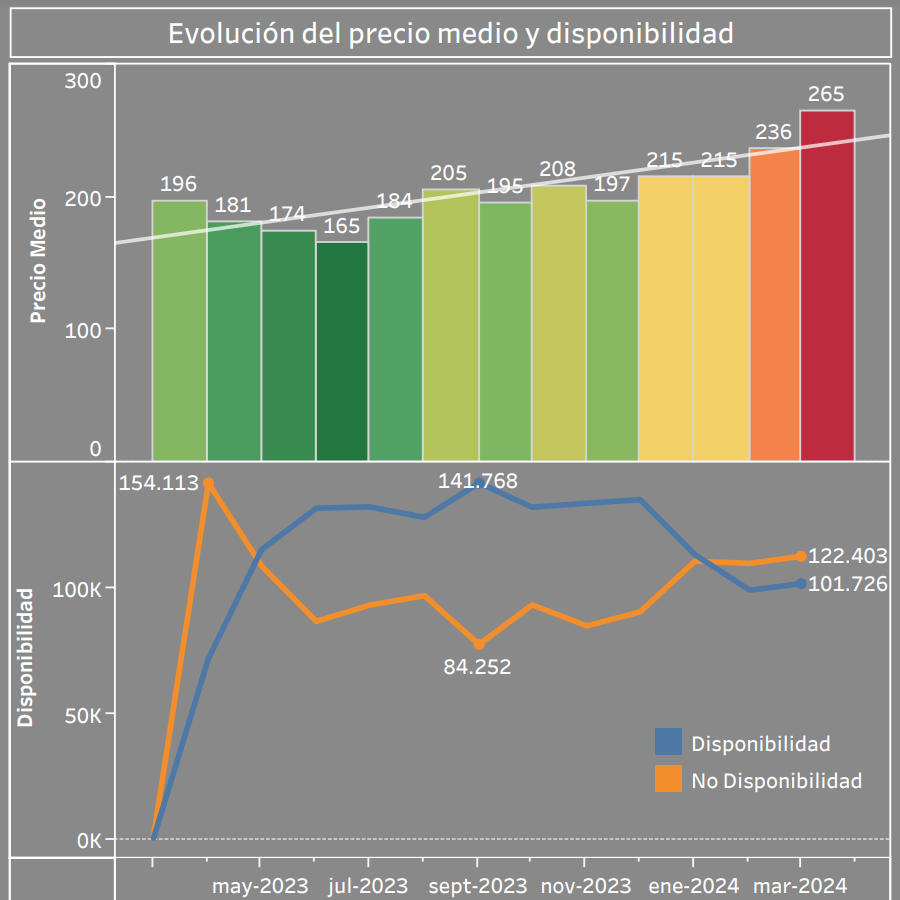
\includegraphics[width=0.7\textwidth]{capturas/18.png}
    \captionof{figure}{Evolución del precio medio y disponibilidad.}
\end{center}
 En algunos meses, como abril, mayo y junio, la disponibilidad es más alta, lo que puede indicar una mayor demanda durante las temporadas turísticas o vacacionales. Por otro lado, en meses como enero y febrero, la disponibilidad tiende a ser más baja, lo que podría relacionarse con la temporada baja después del invierno en la ciudad.
 \newpage
Vamos a analizar en detalle la relación entre las valoraciones y las reseñas en diferentes aspectos. A continuación, se presentan una serie de gráficas que nos proporcionan información valiosa sobre las tendencias en función de las valoraciones y reseñas:
\begin{center}
    \centering
    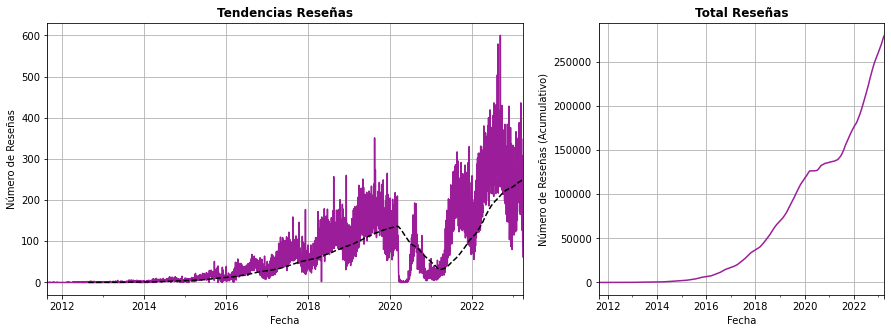
\includegraphics[width=1\textwidth]{capturas/20.png}
    \captionof{figure}{Reseñas a lo largo de los años.}
\end{center}
Se observa un patrón de crecimiento constante, con un notable aumento a partir de 2018. Este aumento puede ser atribuido al aumento de la popularidad de plataformas como Airbnb. Sin embargo, en 2020, se observa una disminución marcada en las reseñas, posiblemente debido a la pandemia de COVID-19 que afectó los viajes y la hospitalidad. A partir de 2021, las reseñas vuelven a aumentar, lo que sugiere una recuperación en el sector.
\begin{center}
    \centering
    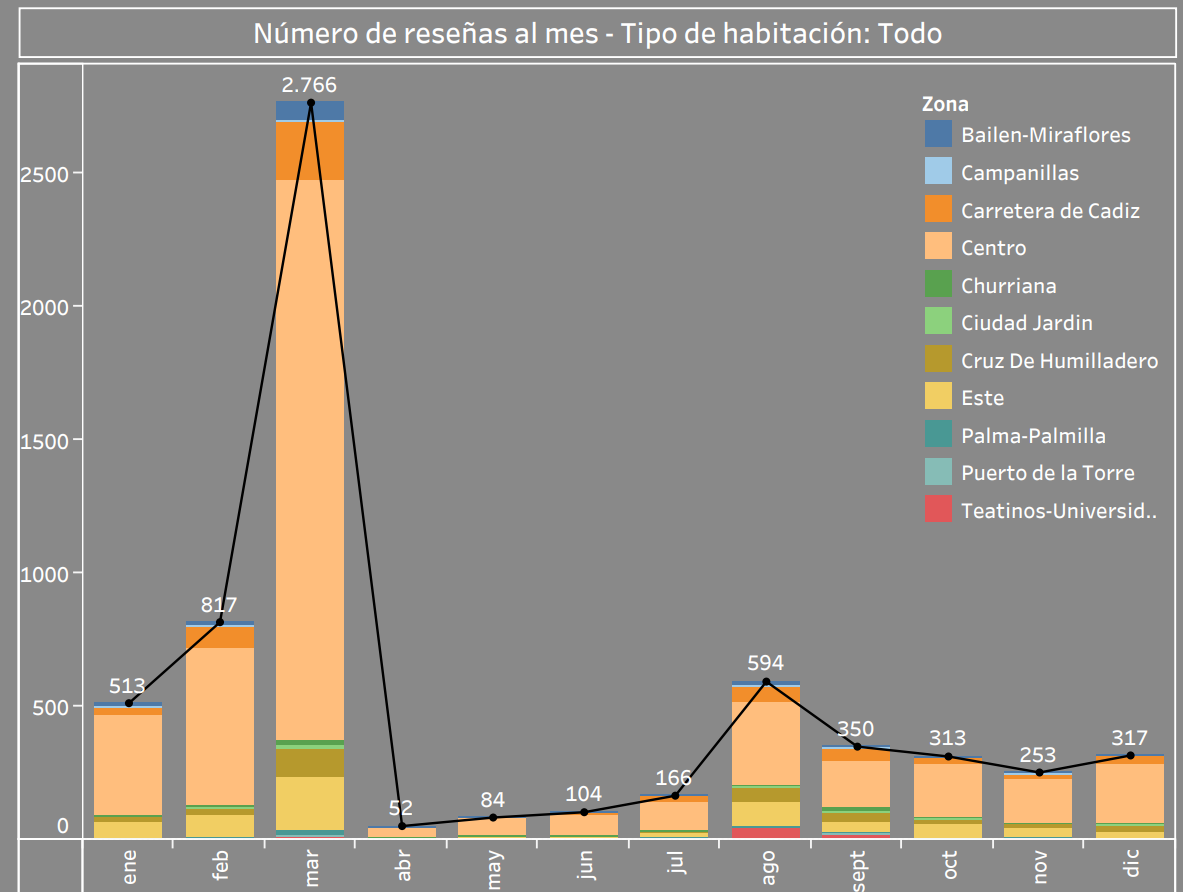
\includegraphics[width=0.8\textwidth]{capturas/22.png}
    \captionof{figure}{Promedio de reseñas por mes.}
\end{center}
Esta gráfica muestra el promedio de reseñas por mes y por barrio. Resalta que en marzo, el número promedio de reseñas es más alto, alcanzando un pico de 2766 reseñas en ese mes. Además, se observa que el distrito \textit{Centro} tiene la mayoría de las reseñas, pues es donde se sitúan la mayoría de alojamientos.
\begin{center}
    \centering
    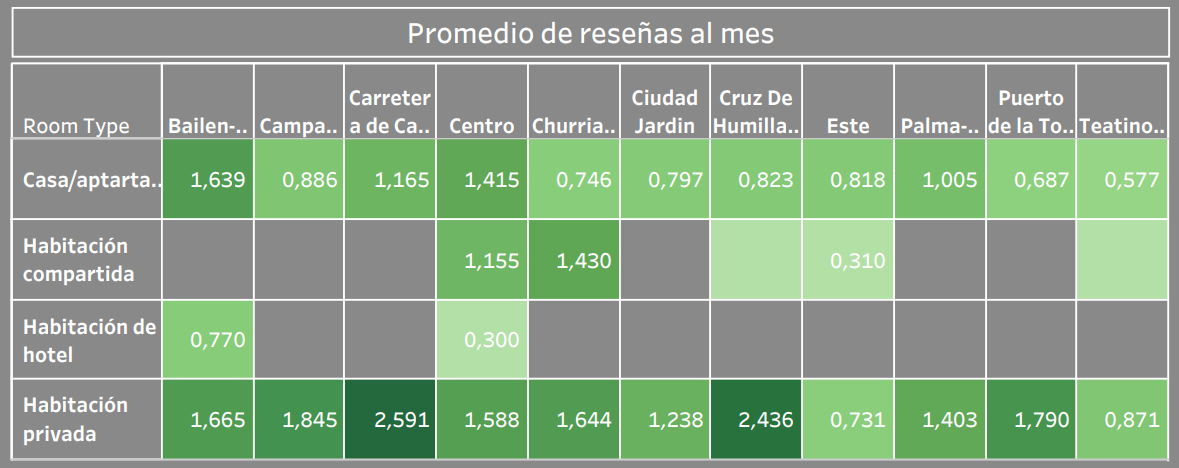
\includegraphics[width=0.8\textwidth]{capturas/24.png}
    \captionof{figure}{Promedio de reseñas por mes por tipo de habitación en cada Zona.}
\end{center}
Se presenta un gráfico que muestra el promedio de reseñas por mes y por tipo de habitación en cada zona. Se puede notar que en el distrito \textit{Carretera de Cádiz} y \textit{Cruz de Humilladero}, las habitaciones privadas tienen una mayor cantidad de reseñas en comparación con otros tipos de habitaciones. Esto podría indicar que estas zonas son preferidas por los huéspedes que buscan habitaciones privadas en lugar de alquileres completos o compartidos.

\subsection{Vista de los alojamientos mejor valorados por categoría de propiedad}

Se creó una vista llamada 'top\_rated\_listings' para mostrar los alojamientos mejor valorados por categoría de propiedad. Esta información puede ser de gran interés para los viajeros que buscan opciones de alojamiento con altas valoraciones por parte de otros usuarios. \\
A continuación se muestra el código de la vista y un fragmento de los resultados:

\begin{verbatim}
CREATE OR REPLACE VIEW top_rated_listings AS
	SELECT listing_url, property_type, name, review_scores_rating
	FROM listings
	WHERE review_scores_rating IS NOT NULL
	ORDER BY review_scores_rating DESC;
\end{verbatim}

\begin{table}[h]
\centering
\resizebox{\textwidth}{!}{
\begin{tabular}{|l|l|l|r|}
\hline
\textbf{Enlace del Alojamiento} & \textbf{Tipo de Propiedad} & \textbf{Nombre} & \textbf{Valoración} \\ \hline
\href{https://www.airbnb.com/rooms/25233010}{https://www.airbnb.com/rooms/25233010} & Entire loft & GUADALMAR SEA\&GOLF & 5 \\ \hline
\href{https://www.airbnb.com/rooms/33438511}{https://www.airbnb.com/rooms/33438511} & Entire rental unit & MALAGUETA PLAYA AZUL MEDITERRANEO & 5 \\ \hline
\href{https://www.airbnb.com/rooms/33422857}{https://www.airbnb.com/rooms/33422857} & Entire rental unit & Apartamento Las Dalias, Málaga, Costa del sol. & 5 \\ \hline
\href{https://www.airbnb.com/rooms/41525349}{https://www.airbnb.com/rooms/41525349} & Room in boutique hotel & Hotel Del Pintor, Habitación económica & 5 \\ \hline
\href{https://www.airbnb.com/rooms/33073492}{https://www.airbnb.com/rooms/33073492} & Entire rental unit & VILLA CANDADO PRIVATE SWIMMING POOL & 5 \\ \hline
\href{https://www.airbnb.com/rooms/34592596}{https://www.airbnb.com/rooms/34592596} & Entire home & Playa 45, first line beach house in El Palo Málaga & 5 \\ \hline
\href{https://www.airbnb.com/rooms/34515076}{https://www.airbnb.com/rooms/34515076} & Entire rental unit & Studio Arts Malaga-Soho & 5 \\ \hline
\href{https://www.airbnb.com/rooms/33728797}{https://www.airbnb.com/rooms/33728797} & Entire rental unit & Apartamento Palma & 5 \\ \hline
\href{https://www.airbnb.com/rooms/33108239}{https://www.airbnb.com/rooms/33108239} & Entire rental unit & Apartamento El Marqués 6 San Juan 1 & 5 \\ \hline
... & ... & ... & ... \\ \hline
\end{tabular}
}
\caption{Alojamientos mejor valorados por categoría de propiedad.}
\end{table}
Si consultamos la vista desde la última fila observaremos los alojamientos con peor valoración. Esto puede ser útil para los viajeros que desean evitar opciones con calificaciones bajas y asegurarse de tener una experiencia positiva durante su estancia.

\begin{table}[h]
\centering
\resizebox{\textwidth}{!}{
\begin{tabular}{|l|l|l|r|}
\hline
\textbf{Enlace} & \textbf{Tipo de Propiedad} & \textbf{Nombre} & \textbf{Valoración} \\ \hline
\href{https://www.airbnb.com/rooms/24762693}{https://www.airbnb.com/rooms/24762693} & Entire home & Apartamento en centro de Málaga & 0 \\ \hline
\href{https://www.airbnb.com/rooms/41375127}{https://www.airbnb.com/rooms/41375127} & Entire loft & Loft Larios, único y exclusivo, repetirás! & 0 \\ \hline
\href{https://www.airbnb.com/rooms/41902864}{https://www.airbnb.com/rooms/41902864} & Entire rental unit & Camino Suárez 2 & 0 \\ \hline
\href{https://www.airbnb.com/rooms/50916471}{https://www.airbnb.com/rooms/50916471} & Entire rental unit & Holidays2Malaga Reyna Manescau - Huelin Area just 450 mts from beach & 1 \\ \hline
\href{https://www.airbnb.com/rooms/702141724072577174}{https://www.airbnb.com/rooms/702141724072577174} & Entire rental unit & "Nuevo apartamento Catedral (centro Málaga)" & 1 \\ \hline
... & ... & ... & ... \\ \hline
\end{tabular}
}
\caption{Alojamientos peor valorados por categoría de propiedad.}
\end{table}

\subsection{Vista de los alojamientos con comentarios negativos}

Se creó una vista llamada 'negative\_reviews' para mostrar los alojamientos con comentarios negativos. Los comentarios son extraídos de la tabla de reseñas y se comparan con palabras clave que podrían indicar aspectos negativos de la estancia, como suciedad, desorden o ruido.\\A continuación se muestra el código de la vista.

\begin{verbatim}
CREATE OR REPLACE VIEW negative_reviews AS
    SELECT li.host_name, li.listing_url, li.host_id, li.host_url,
        r.comments
    FROM reviews r
    JOIN listings li ON r.listing_id = li.id
    WHERE r.comments LIKE '%sucio%' OR
          r.comments LIKE '%desordenado%' OR
          r.comments LIKE '%ruidoso%'
    ORDER BY li.id;
\end{verbatim}
Al revisar esta vista, los anfitriones y propietarios pueden identificar áreas de mejora y tomar medidas para brindar una estancia más satisfactoria a sus huéspedes en el futuro. Además, los viajeros pueden usar esta información para tomar decisiones informadas al elegir su alojamiento, evitando potenciales problemas y asegurando una experiencia positiva durante su estancia en Málaga.

\subsection{Vista de los propietarios con más reseñas con comentarios negativos}

Se creó una vista llamada 'owner\_negative\_reviews' para mostrar los propietarios con más reseñas con comentarios negativos. Esta vista se ha creado para identificar a los propietarios que han recibido más comentarios negativos en sus alojamientos, lo que puede ser útil para tomar decisiones informadas al seleccionar un lugar para hospedarse. \\A continuación se muestra el código de la vista y un fragmento de los resultados:

\begin{verbatim}
CREATE OR REPLACE VIEW owner_negative_reviews AS
    SELECT li.host_name, li.host_url, COUNT(*) 
        AS negative_review_count
    FROM reviews r
    JOIN listings li ON r.listing_id = li.id
    WHERE r.comments LIKE '%sucio%' OR
          r.comments LIKE '%desordenado%' OR
          r.comments LIKE '%ruidoso%'
    GROUP BY li.host_name, li.host_id, li.host_url
    ORDER BY negative_review_count DESC;
\end{verbatim}
\begin{center}
\resizebox{\textwidth}{!}{
\begin{tabular}{|l|l|l|}
\hline
\textbf{Propietario} & \textbf{Enlace del Propietario} & \textbf{Cantidad de Reseñas Negativas} \\ \hline
Malaga & \href{https://www.airbnb.com/users/show/252959314}{https://www.airbnb.com/users/show/252959314} & 18 \\ \hline
Homeabout & \href{https://www.airbnb.com/users/show/17499500}{https://www.airbnb.com/users/show/17499500} & 17 \\ \hline
MimoRooms & \href{https://www.airbnb.com/users/show/7082899}{https://www.airbnb.com/users/show/7082899} & 16 \\ \hline
Urbe10 & \href{https://www.airbnb.com/users/show/151527355}{https://www.airbnb.com/users/show/151527355} & 14 \\ \hline
Ana & \href{https://www.airbnb.com/users/show/9744958}{https://www.airbnb.com/users/show/9744958} & 11 \\ \hline
Alberto & \href{https://www.airbnb.com/users/show/138864019}{https://www.airbnb.com/users/show/138864019} & 11 \\ \hline
Welcome & \href{https://www.airbnb.com/users/show/329266025}{https://www.airbnb.com/users/show/329266025} & 11 \\ \hline
Antonio. & \href{https://www.airbnb.com/users/show/89705945}{https://www.airbnb.com/users/show/89705945} & 10 \\ \hline
Vintage Flat & \href{https://www.airbnb.com/users/show/324236176}{https://www.airbnb.com/users/show/324236176} & 9 \\ \hline
La Recepción & \href{https://www.airbnb.com/users/show/5890675}{https://www.airbnb.com/users/show/5890675} & 9 \\ \hline
Casa Ale & \href{https://www.airbnb.com/users/show/82314525}{https://www.airbnb.com/users/show/82314525} & 9 \\ \hline
Mariano & \href{https://www.airbnb.com/users/show/3301281}{https://www.airbnb.com/users/show/3301281} & 9 \\ \hline
Remy & \href{https://www.airbnb.com/users/show/278821830}{https://www.airbnb.com/users/show/278821830} & 9 \\ \hline
Lu\&Cia & \href{https://www.airbnb.com/users/show/126386697}{https://www.airbnb.com/users/show/126386697} & 9 \\ \hline
.. & ... & ... \\ \hline
\end{tabular}
}
\end{center}
Al analizar esta vista, podemos identificar a los propietarios que pueden tener problemas recurrentes en sus propiedades y evitar potenciales experiencias desagradables.
\newpage
